\section{Vector spaces}

    \newdef{$K$-vector space}{\label{linalgebra:vector_space}
        Let $K$ be a field. A $K$-vector space $V$ is a set equipped with two operations, \textbf{addition} $V\times V\rightarrow V$ and \textbf{scalar multiplication} $K\times V\rightarrow V$, that satisfy the following axioms:
        \begin{enumerate}
            \item $V$ forms an Abelian group under vector addition.
            \item Scalar multiplication is associative: $\lambda(\mu v) = (\lambda\mu)v$ for all $\lambda,\mu\in K$ and $v\in V$.
            \item The identity of the field $K$ acts as a neutral element for scalar multiplication: $1_Kv = v$ for all $v\in V$.
            \item Scalar multiplication is distributive with respect to vector addition: $\lambda(v + w) = \lambda v + \lambda w$ for all $\lambda\in K$ and $v,w\in V$.
        \end{enumerate}
    }
    From here on the underlying field $K$ will be left implicit unless the results depend on it.

\subsection{Linear independence}

    \newdef{Linear combination}{\label{linalgebra:linear_combination}
        The vector $w$ is a linear combination of elements in the set $\{v_i\}_{i\leq n}$ if it can be written as
        \begin{gather}
            w = \sum_{i=1}^n\lambda_i v_i
        \end{gather}
        for some $\{\lambda_i\}_{i\leq n}\subset K$. One can generalize this to general subsets $S\subseteq V$, but the number of nonzero elements $\lambda_i$ is always required to be finite.\footnote{Generalizations are possible in the context of topological vector spaces (see Chapters \ref{chapter:topology} and \ref{chapter:normed_spaces}), where one can define the notion of convergence.}
    }
    \newdef{Linear independence}{\label{linalgebra:linear_independence}
        A finite set $\{v_i\}_{i\leq n}$ is said to be linearly independent if the following relation holds:
        \begin{gather}
            \sum_{i=1}^n\lambda_i v_i = 0 \iff \forall i\leq n:\lambda_i = 0.
        \end{gather}
        A general set $S\subset V$ is linearly independent if every finite subset of it is linearly independent.
    }

    \newdef{Span}{\index{span}
        A set of vectors $S\subseteq V$ is said to span $V$ if every vector $v\in V$ can be written as a linear combination of elements in $S$.
    }

    \newdef{Frame}{\index{frame}
        A $k$-frame is an ordered set of $k$ linearly independent vectors.
    }

\subsection{Bases}

    \newdef{Basis}{
        A set $\mathcal{B}$ is said to be a basis of $V$ if $\mathcal{B}$ is linearly independent and if it spans $V$.
    }
    \begin{property}
        Every spanning set contains a basis.
    \end{property}

    \begin{remark}\index{basis!Schauder}
        In the previous definition the concept of a \textit{Hamel} basis was implicitly used. This concept is based on two conditions:
        \begin{enumerate}
            \item The basis is linearly independent.
            \item Every element in the vector space can be written as a linear combination of a \underline{finite} subset of the basis. (See the footnote above.)
        \end{enumerate}
        For bases consisting of a finite number of vectors, one does not have to worry. For infinite bases one has to keep this in mind. An alternative construction, which allows for combinations of a countably infinite number of elements, is given by that of a \textit{Schauder basis}. However, it can be shown that every vector space admits a Hamel basis:
    \end{remark}
    \begin{construct}[\difficult{Hamel basis}]\index{basis!Hamel}\label{linalgebra:hamel_basis}
        Let $V$ be a vector space and consider the set of all linearly independent subsets of $V$. Under the relation of inclusion this set becomes a partially ordered set \ref{set:poset}. Zorn's lemma \ref{set:zorns_lemma} then says that there exists at least one maximal linearly independent set.

        Now, one can show that this maximal subset $S$ is also a spanning set of $V$. Choose a vector $v\in V$ that is not already in $S$. From the maximality of $S$ it follows that $S\cup v$ is linearly dependent and hence there exists a finite sequence of scalars $(a^1,\ldots,a^n,b)$ and a finite sequence of elements $(e_1,\ldots,e_n)$ in $S$ such that:
        \begin{gather}
            \sum_{i=0}^n a^ie_i + bv = 0,
        \end{gather}
        where not all scalars are zero. This then implies that $b\neq0$, because otherwise the set $\{e_i\}_{i\leq n}$ and hence also $S$ would be linearly dependent. It follows that $v$ can be written as\footnote{It is this step that requires $R$ to be a division ring in Property \ref{algebra:module_basis} because otherwise we would not generally be able to divide by $b\in R$.}
        \begin{gather}
            v = -\frac{1}{b}\sum_{i=0}^na^ie_i.
        \end{gather}
        Because $v$ was randomly chosen, one can conclude that $S$ is a spanning set for $V$.
    \end{construct}
    \begin{remark*}
        This construction clearly assumes the axiom of choice in set theory, only ZF does not suffice. It can even be shown that the existence of a Hamel basis for every vector space is equivalent to the axiom of choice (and thus also Zorn's lemma).
    \end{remark*}

    \begin{property}
        Every basis of $V$ has the same number of elements. For infinite-dimensional spaces this means that all bases have the same \textit{cardinality}.
    \end{property}
    \newdef{Dimension}{\index{dimension}\label{linalgebra:dimension}
        Let $V$ be a finite-dimensional vector space and let $\mathcal{B}$ be a basis for $V$ that contains $n$ elements. With the previous property in mind, the dimension of $V$ is defined as follows:
        \begin{gather}
            \dim(V) := n.
        \end{gather}
    }

    \newdef{Subspace}{\label{linalgebra:subspace}
        Let $V$ be a vector space. A subset $W$ of $V$ is a subspace if $W$ is itself a vector space under (the restriction of) the operations of $V$:
        \begin{gather}
            W \leq V\iff\forall w_1,w_2\in W,\forall\lambda\in K:\lambda w_1 + w_2 \in W.
        \end{gather}
    }

\subsection{Sum and direct sum}

    \newdef{Sum}{\index{sum}
        \nomenclature[O_zsymbinsum]{$X+Y$}{Sum of the vector spaces $X$ and $Y$.}
        Let $V$ be a vector space and consider a collection of subspaces $\{W_1,\ldots,W_k\}$. The sum of these subspaces is defined as follows:
        \begin{gather}
            W_1+\cdots+W_k := \left\{\sum_{i=1}^kw_i\,\middle\vert\,w_i\in W_i\right\}.
        \end{gather}
    }
    \newdef{Direct sum}{\index{direct!sum}\label{linalgebra:direct_sum}
        \nomenclature[O_zsymbinsump]{$X\oplus Y$}{Direct sum of the vector spaces $X$ and $Y$.}
        If every element $v$ of the sum can be written as a unique linear combination, the sum is called a direct sum.
    }
    \newnot{Direct sum}{
        The direct sum of vector spaces is denoted by
        \begin{gather*}
            W_1\oplus\cdots\oplus W_k\equiv\bigoplus_{i=1}^kW_i.
        \end{gather*}
    }

    \begin{formula}
        Let $V$ be a finite-dimensional vector space and consider two subspaces $W_1,W_2\leq V$. The dimensions of these spaces can be related in the following way:
        \begin{gather}
            \dim(W_1 + W_2) = \dim(W_1) + \dim(W_2) - \dim(W_1\cap W_2).
        \end{gather}
    \end{formula}
    \begin{property}
        Let $V$ be a vector space and assume that $V$ can be decomposed as $W=W_1\oplus W_2$. If $\mathcal{B}_1$ is a basis of $W_1$ and if $\mathcal{B}_2$ is a basis of $W_2$, then $\mathcal{B}_1\cup\mathcal{B}_2$ is a basis of $W$.
    \end{property}

    \newdef{Complement}{\index{complement}
        Let $V$ be a vector space and let $W$ be a subspace of $V$. A subspace $W'$ of $V$ is called a complement of $W$ if $V = W\oplus W'$.
    }
    \begin{property}[Existence of complements]\label{linalgebra:complement}
        Let $V$ be a vector space and let $U,W$ be two subspaces of $V$. If $V = U+W$, there exists a subspace $Y\leq U$ such that $V = Y\oplus W$. Furthermore, every subspace of $V$ has a complement in $V$.
    \end{property}

\subsection{Algebras}

    \newdef{Algebra}{\index{algebra}\label{linalgebra:algebra}
        Let $V$ be a vector space equipped with a binary operation $\star:V\times V\rightarrow V$. The pair $(V,\star)$ is called an algebra over $K$ if it satisfies the following conditions:
        \begin{enumerate}
            \item \textbf{Right distributivity}: $(x + y)\star z = x\star z + y\star z$,
            \item \textbf{Left distributivity}: $x\star(y + z) = x\star y + x\star z$, and
            \item \textbf{Compatibility with scalars}: $(\lambda x)\star(\mu y) = \lambda\mu(x\star y)$.
        \end{enumerate}
        These conditions say that the binary operation is bilinear. An algebra $V$ is said to be unital if it contains an identity element with respect to the bilinear map $\star$.
    }

    \remark{More generally one can define an algebra over a commutative unital ring $R$. The defining conditions remain the same, except that one requires $V$ to be an $R$-module instead of a vector space.}

    \newdef{Division algebra}{\index{division!algebra}
        A unital algebra in which every nonzero element has both a left and right multiplicative inverse. If the algebra is associative, these inverses coincide. A normed division algebra is a division algebra equipped with a multiplicative quadratic form $q$ such that $\langle a|b \rangle := \frac{1}{2}[q(a+b)-q(a)-q(b)]$ is a nondegenerate inner product \ref{linalgebra:innerproduct}.
    }
    \begin{theorem}[Frobenius]\index{Frobenius}
        There exist three inequivalent finite-dimensional real associative division algebras: $\mathbb{R},\mathbb{C}$ and $\mathbb{H}$.
    \end{theorem}
    \begin{theorem}[Hurwitz]\index{Hurwitz}\label{linalgebra:hurwitz}
        There exist four inequivalent finite-dimensional real normed division algebras: $\mathbb{R},\mathbb{C},\mathbb{H}$ and $\mathbb{O}$.
    \end{theorem}

    \begin{example}[Frobenius algebra]\index{Frobenius!algebra}\label{linalgebra:frobenius}
        An algebra $A$ equipped with a nondegenerate bilinear form $\eta:A\times A\rightarrow A$ satisfying the following condition for all $a,b,c\in A$:
        \begin{gather}
            \eta(ab,c)=\eta(a,bc).
        \end{gather}
    \end{example}

    \begin{example}[Temperley-Lieb algebra]\index{Temperley-Lieb algebra}\index{Jones!relations}
        \nomenclature[S_TLn]{$\text{TL}_n(\delta)$}{Temperley-Lieb algebra with $n-1$ generators and parameter $\delta$.}
        Let $R$ be a commutative unital ring and fix an element $\delta\in R$. The Temperley-Lieb algebra $\text{TL}_n(\delta)$ is the unital $R$-algebra with generators $\{U_i\}_{i<n}$ that satisfy the \textbf{Jones relations}:
        \begin{enumerate}
            \item $U_i^2 = \delta U_i$,
            \item $U_i U_j = U_j U_i$ if $|i-j|\neq 1$, and
            \item $U_i U_j U_i = U_i$ if $|i-j| = 1$.
        \end{enumerate}
        One can represent the elements of a Temperley-Lieb algebra diagrammatically. All elements of $\text{TL}_n(\delta)$ are represented as diagrams with $n$ inputs and $n$ outputs:

        \qquad The unit is given by the diagram where all inputs are connected to the outputs directly across the diagram. The generators $\{U_i\}_{i<n}$ are constructed by connecting the $i^{th}$ input (resp. output) to the $i+1^{th}$ input (resp. output) and all other inputs are connected to the output directly across the diagram.
        Multiplication in $\text{TL}_n(\delta)$ is performed diagrammatically by placing two diagrams side by side. Closed loops are replaced by a factor $\delta$.

        \begin{figure}[ht!]
            \centering
            \begin{subfigure}{0.49\textwidth}
                \centering
                
\begin{tikzpicture}
                    \draw (0, 0) -- (2, 0);
                    \draw (0, 0.3) -- (2, 0.3);
                    \draw (0, 0.6) -- (2, 0.6);
                    \draw (0, 0.9) -- (2, 0.9);
                \end{tikzpicture}
                \caption{Unit in TL$_4(\delta)$.}
                \label{fig:unit_temperley_lieb}
            \end{subfigure}
            \begin{subfigure}{0.49\textwidth}
                \centering
                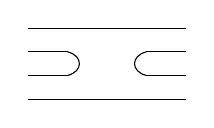
\begin{tikzpicture}
                    \draw (0, 0) -- (2, 0);
                    \draw (0, 0.3) -- (0.5, 0.3);
                    \draw (0, 0.6) -- (0.5, 0.6);
                    \draw (0.5, 0.3) .. controls (0.7, 0.35) and (0.7, 0.55) .. (0.5, 0.6);
                    \draw (1.5, 0.3) -- (2, 0.3);
                    \draw (1.5, 0.6) -- (2, 0.6);
                    \draw (1.5, 0.3) .. controls (1.3, 0.35) and (1.3, 0.55) .. (1.5, 0.6);
                    \draw (0, 0.9) -- (2, 0.9);
                \end{tikzpicture}
                \caption{Generator $U_2$ in $\text{TL}_4(\delta)$.}
                \label{fig:generator_temperley_lieb}
            \end{subfigure}
        \end{figure}
    \end{example}

\section[Linear maps]{Linear maps\footnote{Also called \textbf{linear mapping} or \textbf{linear transformation}.}}
\subsection{Homomorphisms}

    \newdef{Homomorphism space}{\index{morphism!of vector spaces}\label{linalgebra:hom_space}
        \nomenclature[S_Hom]{$\hom(V, W)$}{Space of morphisms from a set $V$ to a set $W$.}
        Let $V,W$ be two vector spaces. The set of all linear maps between $V$ and $W$ is called the homomorphism space from $V$ to $W$, or shorter, the \textbf{hom-space} from $V$ to $W$:
        \begin{gather}
            \hom_K(V, W) := \big\{f:V\rightarrow W\,\big\vert\,f\text{ is linear}\big\}.
        \end{gather}
    }
    \begin{formula}\label{linalgebra:hom_dimension}
        If $V,W$ are two finite-dimensional vector spaces, then
        \begin{gather}
            \dim\left(\hom_K(V,W)\right) =\dim(V)\dim(W).
        \end{gather}
    \end{formula}

    \newdef{Endomorphism ring}{\index{endomorphism}
        \nomenclature[S_End]{$\text{End}(V)$}{Ring of endomorphisms on a set $V$.}
        The space $\hom_K(V,V)$ with composition of maps as multiplication forms a ring, the endomorphism ring. It is denoted by $\text{End}_K(V)$ or $\text{End}(V)$ when the underlying field is clear.
    }
    \begin{property}[Commutator]\index{commutator}
        The endomorphism ring $\text{End}(V)$ forms a Lie algebra (Property \ref{lie:end_as_lie_algebra}) when equipped with the commutator
        \begin{gather}
            [A,B] := A\circ B - B\circ A.
        \end{gather}
    \end{property}

    \begin{property}
        Let $V$ be finite-dimensional vector space and let $f:V\rightarrow V$ be an endomorphism. The following statements are equivalent:
        \begin{itemize}
            \item $f$ is injective.
            \item $f$ is surjective.
            \item $f$ is bijective.
        \end{itemize}
    \end{property}

    \newdef{Automorphism}{\index{automorphism}\index{general linear group}\label{linalgebra:automorphism}
        \nomenclature[S_Aut]{$\text{Aut}(V)$}{group of automorphisms (invertible endomorphisms) of a set $V$}
        \nomenclature[S_GL]{$\text{GL}(V)$}{general linear group: the group of all automorphisms of a vector space $V$}
        An isomorphism from $V$ to $V$ is called an automorphism. The set of all automorphisms  on $V$, which in fact forms a group, is denoted by $\text{Aut}(V)$. In some situations one speaks of the general linear group\footnote{This group is isomorphic to the general linear group of invertible matrices \ref{linalgebra:GL_matrices} (hence the similar name and notation).} $\text{GL}_K(V)$ or $\text{GL}(V)$ when the underlying field is clear.
    }
    \remark{Sometimes automorphisms are also called \textbf{linear operators}. However, this terminology is also used for a general linear map in operator theory (Chapter \ref{chapter:operator_algebras}) and so this term is not adopted in this text.}

    \newdef{Kernel}{\index{kernel}
        Consider a linear map $f:V\rightarrow W$. The kernel of $f$ is defined as the following subspace of $V$:
        \begin{gather}
            \text{ker}(f) := \{v\in V\mid f(v) = 0\}.
        \end{gather}
    }
    \begin{property}
        A linear map $f:V\rightarrow W$ is injective if and only if $\text{ker}(f) = 0$.
    \end{property}

    \newdef{Rank}{\index{rank}\label{linalgebra:image_rank}
        The dimension of the image of a linear map.
    }
    \newdef{Nullity}{\index{nullity}
        The dimension of the kernel of a linear map.
    }

    \begin{theorem}[Dimension theorem\footnotemark]\index{rank-nullity theorem}\label{linalgebra:dimension_theorem}
        \footnotetext{Also called the \textbf{rank-nullity theorem}.}
        Let $f:V\rightarrow W$ be a linear map.
        \begin{gather}
            \dim(\text{\upshape im}(f)) + \dim(\text{\upshape ker}(f)) = \dim(\text{\upshape V})
        \end{gather}
    \end{theorem}
    \begin{result}\label{linalgebra:dimension_isomorphism}
        Two finite-dimensional vector spaces are isomorphic if and only if they have the same dimension.
    \end{result}

    \newdef{Minimal polynomial}{\index{minimal!polynomial}
        Let $f\in\text{End}(V)$ with $V$ a finite-dimensional vector space. The monic polynomial $\mu_f$ of lowest order such that $\mu_f(f)=0$ is called the minimal polynomial of $f$.
    }
    \begin{property}\label{linalgebra:minimal_polynomial_divisor}
        Let $f\in\text{End}(V)$ with minimal polynomial $\mu_f$ and consider a polynomial $\varphi\in K[x]$. If $\varphi(f) = 0$, the minimal polynomial $\mu_f$ divides $\varphi$.
    \end{property}

    \begin{property}[Jordan-Chevalley decomposition]\index{Jordan-Chevalley decomposition}\index{semisimple!operator}\index{nilpotent}\label{linalgebra:jordan_chevalley}
        Every endomorphism $A$ can be decomposed as follows:
        \begin{gather}
            A = A_{ss} + A_n,
        \end{gather}
        where
        \begin{itemize}
            \item $A_{ss}$ is \textbf{semisimple}, i.e. for every invariant subspace of $A_{ss}$ there exists an invariant complementary subspace.
            \item $A_n$ is \textbf{nilpotent}, i.e. $\exists k\in\mathbb{N}: A_n^k = 0$.
        \end{itemize}
        Furthermore, this decomposition is unique and the endomorphisms $A_{ss}, A_n$ can be written as polynomials in $A$.
    \end{property}

\subsection{Dual maps}

    \newdef{Dual space}{\index{dual!space}\index{linear!form}
        Let $V$ be a vector space. The (algebraic) dual $V^*$ of $V$ is defined as the following vector space:
        \begin{gather}
            \label{linalgebra:dual_space}
            V^*:=\text{Hom}_K(V, K)=\big\{f:V\rightarrow K\,\big\vert\,f\text{ is linear}\big\}.
        \end{gather}
        The elements of $V^*$ are called \textbf{linear forms} or (linear) \textbf{functionals}.
    }
    \begin{property}[Dimension]\label{linalgebra:dual_space_dimension}
        From Theorem \ref{linalgebra:hom_dimension} it follows that $\dim(V^*)=\dim(V)$ whenever $V$ is finite-dimensional. If $V$ is infinite-dimensional, this property is \underline{never} valid. In the infinite-dimensional case $\text{card}(V^*)>\text{card}(V)$ always holds.
    \end{property}

    \newdef{Dual basis}{
        Let $\mathcal{B} = \{e_1,e_2,\ldots,e_n\}$ be a basis for a finite-dimensional vector space $V$. One can construct a basis $\mathcal{B}^* = \{\varepsilon_1,\varepsilon_2,\ldots,\varepsilon_n\}$ for $V^*$, called the dual basis of $\mathcal{B}$, as follows:
        \begin{gather}
            \label{linalgebra:dual_basis}
            \varepsilon_i:\sum_{j=1}^na_ie_i\mapsto a_i.
        \end{gather}
        The relation between a basis and its associated dual basis can also be expressed as
        \begin{gather}
            \label{linalgebra:dual_basis_2}
            \varepsilon^i(e_j) = \delta^i_j.
        \end{gather}
    }
    \newdef{Natural pairing}{\index{natural!pairing}\label{linalgebra:natural_pairing}
        The definition of the dual basis extends to a natural pairing of $V$ and its dual $V^*$ in terms of the following bilinear map:
        \begin{gather}
            \langle v, v^*\rangle := v^*(v).
        \end{gather}
        See also \ref{cat:dual} for a generalization of this map.
    }

    \newdef{Dual map}{\index{dual!map}\label{linalgebra:transpose}
        Let $f:V\rightarrow W$ be a linear map. The linear map
        \begin{gather}
            f^*:W^*\rightarrow V^*:\varphi\rightarrow\varphi\circ f
        \end{gather}
        is called the dual map or \textbf{transpose} of $f$.
    }

\subsection{Convexity}

    \newdef{Convex set}{\index{convex}\index{hull}\label{linalgebra:convex}
        A subset of $X$ of a vector space $V$ is said to be convex if $x,y\in X$ implies that $\{\lambda x+(1-\lambda)y\mid\lambda\in[0,1]\}\subset X$. The \textbf{convex hull} of a subset $X$ is defined as the smallest convex subset containing $X$.
    }

    \newdef{Convex function}{
        Let $X$ be a convex subset of $V$. A function $f:X\rightarrow \mathbb{R}$ is said to be convex if for all $x, y\in X$ and $\lambda\in[0,1]$:
        \begin{gather}
            f\big(\lambda x + (1-\lambda)y\big) \leq t\lambda(x) + (1-\lambda)f(y).
        \end{gather}
        For the definition of a \textbf{concave} function the inequality has to be turned around.
    }
    \begin{property}
        A function $f:X\rightarrow\mathbb{R}$ is linear if and only if it is both convex and concave.
    \end{property}

    \begin{theorem}[Karamata's inequality]\index{Karamata}
        Let $I\subset\mathbb{R}$ be an interval and let $f:I\rightarrow\mathbb{R}$ be a convex function. If $(x_1, \ldots, x_n)$ is a tuple that majorizes $(y_1, \ldots, y_n)$, i.e.
        \begin{gather}
            \sum_{i=1}^nx_i = \sum_{i=1}^ny_i
        \end{gather}
        and
        \begin{gather}
            x_{(1)} + \cdots + x_{(k)}\geq y_{(1)} + \cdots + y_{(k)}
        \end{gather}
        $\forall k\leq n$, where $x_{(i)}$ denotes the $i^{th}$ largest element of $(x_1,\ldots,x_n)$, then
        \begin{gather}
            \sum_{i=1}^nf(x_i)\geq \sum_{i=1}^nf(y_i).
        \end{gather}
    \end{theorem}
    The following inequality can be derived directly from the definition of convexity by induction:
    \begin{theorem}[Jensen's inequality]\index{Jensen's inequality}
        Let $f$ be a convex function and consider weights $\{a_i\}_{i\leq n}$ such that $\sum_ia_i=1$. Then Jensen's equality states that
        \begin{gather}
            \label{linalgebra:jensen_inequality}
            f\left(\sum_ia_ix_i\right) \leq \sum_ia_if(x_i).
        \end{gather}
    \end{theorem}